\chapter{Cause specific mortality rates: alcohol dependence}
\label{applications-csmr}

A key assumption of the GBD 2010 study is that there is only one cause leading to death.  This categorical distribution of deaths creates a rate that does not directly correspond to any rate in the compartmental model.  The cause-specific mortality rate (CSMR) assumes that everyone who dies \emph{with} the condition dies \emph{of} the condition.  While this is a reasonable assumption for many conditions such as cirrhosis, diarrhea or transport injuries, it is not for conditions such as Parkinson's disease or alcohol dependence.

Alcohol dependence is the dysfunctional pattern of alcohol consumption that leads to physiological dependence and impaired control.  Like cannabis dependence in Chapter \ref{applications-splines_knot_loc}, to be diagnosed with alcohol dependence, three of more of the seven substance dependence criteria defined by the American Psychiatric Association on \pageref{tab:app-substance_dependence} must be fulfilled. \cite{american_diagnostic_2000, hasin_prevalence_2007}  Systematic review yielded prevalence, excess mortality and cause-specific mortality data as seen in Figure \ref{fig:app-alcohol data}.

    \begin{figure}[h]
        \begin{center}
            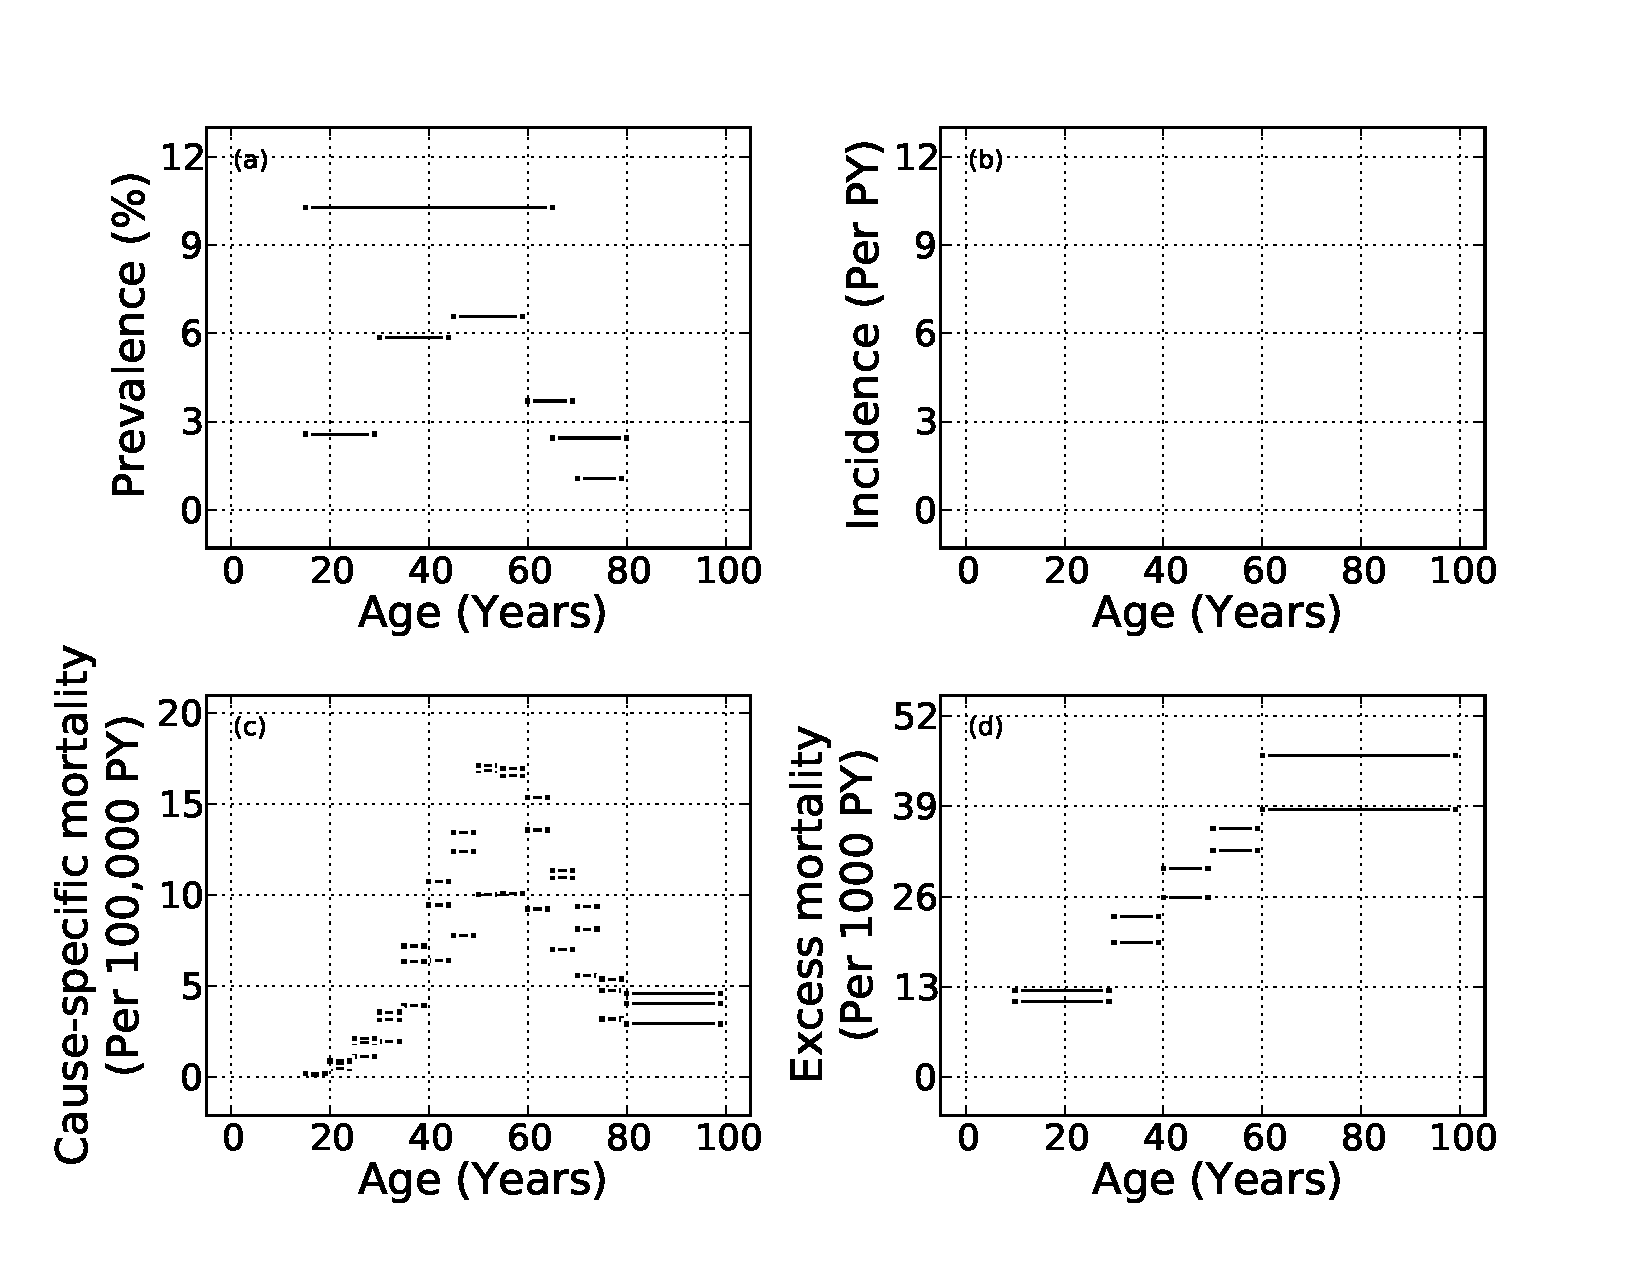
\includegraphics[width=\textwidth]{alcohol-data.pdf}
            \caption{Prevalence (panel (a)), incidence (panel (b)), cause-specific mortality (panel (c)) and excess mortality (panel (d)) of alcohol dependence in Western European males in 2005.}
            \label{fig:app-alcohol data}
        \end{center}
    \end{figure} 

As explained in \ref{sys-dynamics}, excess mortality, $h_{f}$, is the hazard for individuals with the condition.  Theoretically, CSMR may be included in the compartmental model by splitting excess mortality into two parts,
    \begin{equation}
        h_{f} = h_{f''} + h_{f'}
    \end{equation}
where h_{f'} is the excess mortality caused directly by the disease and h_{f''} is the ``excess excess mortality''--the elevated mortality among individuals with the condition.  However, in practice $h_{f''}$ and $h_{f'}$ are never disentangled.  This method implicitly separates $h_{f'}$ and $h_{f''}$ but does not try to explicitly represent both.

TK: better discussion on how $h_{f'}$ related to $h_{pf}$ and $h_{f''}$ to csmr...

CSMR is the lower bound of $h_{pf}$, the product of prevalence and excess mortality.  $h_{pf}$ assumes that deaths \emph{with} the condition are deaths caused \emph{by} the condition.  Therefore, hazard data of this type are treated as a direct measurement of $h_{pf}$.  
\ref{theory-csmr}

    
    \begin{figure}[h]
        \begin{center}
            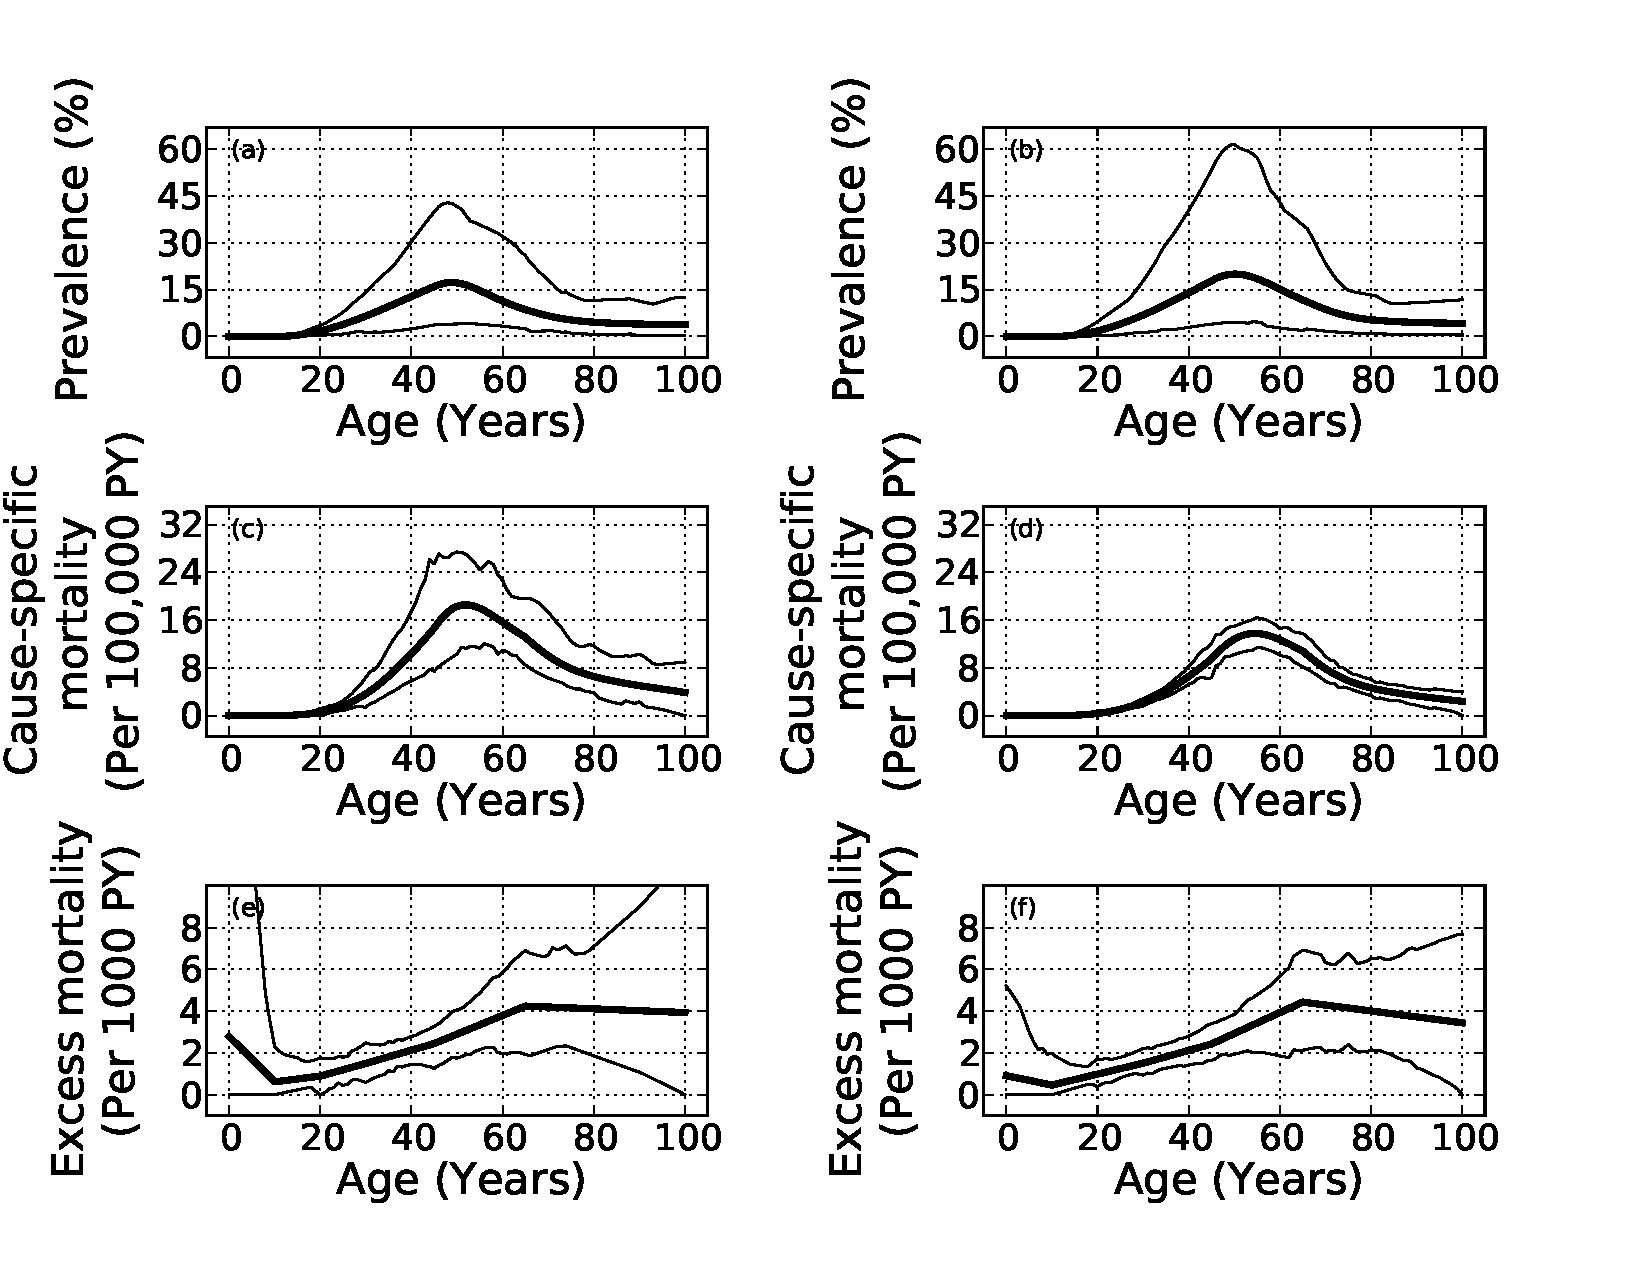
\includegraphics[width=\textwidth]{alcohol-csmr_v_pf.pdf}
            \caption{Prevalence (panel (a)), cause-specific mortality (panel (b)) and excess mortality (panel (d)) of alcohol dependence in Western European males in 2005.}
            \label{fig:app-alcohol compare}
        \end{center}
    \end{figure} 